\documentclass[tcn = 37075, sheet = true, abstract = true]{mcmthesis}
\problem{A}
\usepackage{palatino}
\usepackage{mwe}
\usepackage{slashbox}
\usepackage{algorithm2e}
\usepackage{mathrsfs}
\usepackage{xcolor}

\title{Understanding Employee Churn based on Information Accumulation and Bayesian Learning}
\author{\small \href{http://www.latexstudio.net/}
  {
\includegraphics[width=7cm]{mcmthesis-logo}}}
\date{\today}

\begin{document}
\begin{abstract}
\lipsum[1]
\begin{keywords}
keyword1; keyword2
\end{keywords}
\end{abstract}
\maketitle
\newpage


\tableofcontents
\newpage
\section{Introduction}

\section{Preliminaries}

\subsection{Allocation of Levels of Positions}

(\textit{This paragraph needs rephrasing later}) Building the organizing network of the company requires first to plausibly incorporating the organizational graph (as presented in figure 1) and the allocation of different levels of positions (as indicated in table 1). To reach this, we assign different positions to different offices according to several rules. After some minor adjustments, we can get a possible and reasonable allocation of staff, on which we will build our later analysis. The assumptions related to the allocation are as follows:

\noindent \textbf{Assumptions}:

To explain the assumptions clearly, we first define terms "tree" and "tier". Tree is defined to be the whole picture of the organizational graph. Entries are defined to be in the same tier if they are on the same horizontal line in figure 1. Thus we can see that the tree stems from the higher tier of CEO to the lowest tier of branches. Now the assumptions:

\begin{itemize}
\item Every senior/junior manager should have a clerk in his/her office for administrative tasks.
\item The level of position of a staff tend to be higher when his office is closer to the CEO in the organizational graph.
\item The level of position of a staff tend to be higher when his office is the root of divisions of more people.
\item The level of position of a manager cannot be lower than someone whose office belongs to a lower tier.
\item Research tasks should be conducted by experienced employees.
\end{itemize}

Thus we can get the following table of allocation of 370 positions:
\begin{table}[htb!]
\centering
\begin{tabular}{l|lllllllll}   \hline
\backslashbox{Tier}{}& \backslashbox{Position}{level}&1&2&3&4&5&6&7&Total\\ \hline
1                  & CEO              & 2              & 0              & 0                      & 0                        & 0                    & 0                      & 2                    & 4     \\
\multirow{7}{2pt}{2} & Research           & 1              & 0              & 0                      & 0                        & 2                    & 0                      & 1                    & 4     \\
                   & CIO                & 1              & 2              & 0                      & 0                        & 8                    & 0                      & 3                    & 14    \\
                   & CFO                & 1              & 2              & 0                      & 0                        & 8                    & 0                      & 3                    & 14    \\
                   & HR                 & 0              & 1              & 0                      & 0                        & 2                    & 0                      & 1                    & 4     \\
                   & VP                 & 2              & 0              & 0                      & 0                        & 0                    & 0                      & 2                    & 4     \\
                   & Facilities         & 1              & 0              & 0                      & 0                        & 2                    & 0                      & 1                    & 4     \\
                   & Sales Marketing    & 1              & 0              & 0                      & 0                        & 2                    & 0                      & 1                    & 4     \\
 \multirow{9}{2pt}{3} & Networks           & 0              & 1              & 1                      & 0                        & 11                   & 0                      & 1                    & 14    \\
                   & Information        & 0              & 1              & 1                      & 0                        & 11                   & 0                      & 1                    & 14    \\
                   & Program Manager    & 0              & 1              & 1                      & 0                        & 6                    & 5                      & 1                    & 14    \\
                   & Production Manager & 1              & 1              & 0                      & 0                        & 10                   & 0                      & 2                    & 14    \\
                   & Plant Blue         & 0              & 1              & 1                      & 0                        & 6                    & 5                      & 1                    & 14    \\
                   & Plant Green        & 0              & 1              & 1                      & 0                        & 6                    & 5                      & 1                    & 14    \\
                   & Regional           & 0              & 1              & 1                      & 0                        & 6                    & 5                      & 1                    & 14    \\
                   & World Wide         & 0              & 1              & 1                      & 0                        & 6                    & 5                      & 1                    & 14    \\
                   & Internet           & 0              & 1              & 1                      & 0                        & 6                    & 5                      & 1                    & 14    \\
4                  & Director           & 0              & 6              & 6                      & 0                        & 6                    & 0                      & 6                    & 24    \\
5                  & Branch             & 0              & 0              & 11                     & 25                       & 12                   & 120                    & 0                    & 168   \\ \hline

&Total              & 10             & 20             & 25                     & 25                       & 110                  & 150                    & 30                   & 370 \\  \hline
\end{tabular} 

*1:Senior Manager 2:Junior Manager 3:Experienced Supervisor 4:Inexperienced Supervisor 5:Experienced Employee 6:Inexperienced Employee 7:Administrative Clerk

\caption{The distribution of staff in different positions}
\end{table}

\subsection{Building up Information Network}

We set up to build the information network in this company. Define $V(G)=\{v_1,v_2,...v_{370}\}$ as the set of all positions. Each node denotes one position. Define $E(G)$ as the set of edges in the network. $(v_i,v_j)\in E(G)$ if at least one of the following holds:


\begin{itemize}
\item $i$ and $j$ are in the same office. Here one entry in figure 1 is considered as an office, whether it consists of two divisions of 14 staff members or only four staff members.
\item $i$ is the head of an office and $j$ is the head of the directly-related upper office or the opposite. Here the staff member in the highest level of position within an office is considered as the head of the office, such as the junior manager in Networks office and the experienced supervisor in Branch office.
\item $i$ and $j$ are both senior manager or junior manager.
\end{itemize}

$G=\{V(G),E(G)\}$ is the the graph of this network. We then visualize the network in the following picture (figure 1).

\begin{figure}[htb!]
\small
\centering
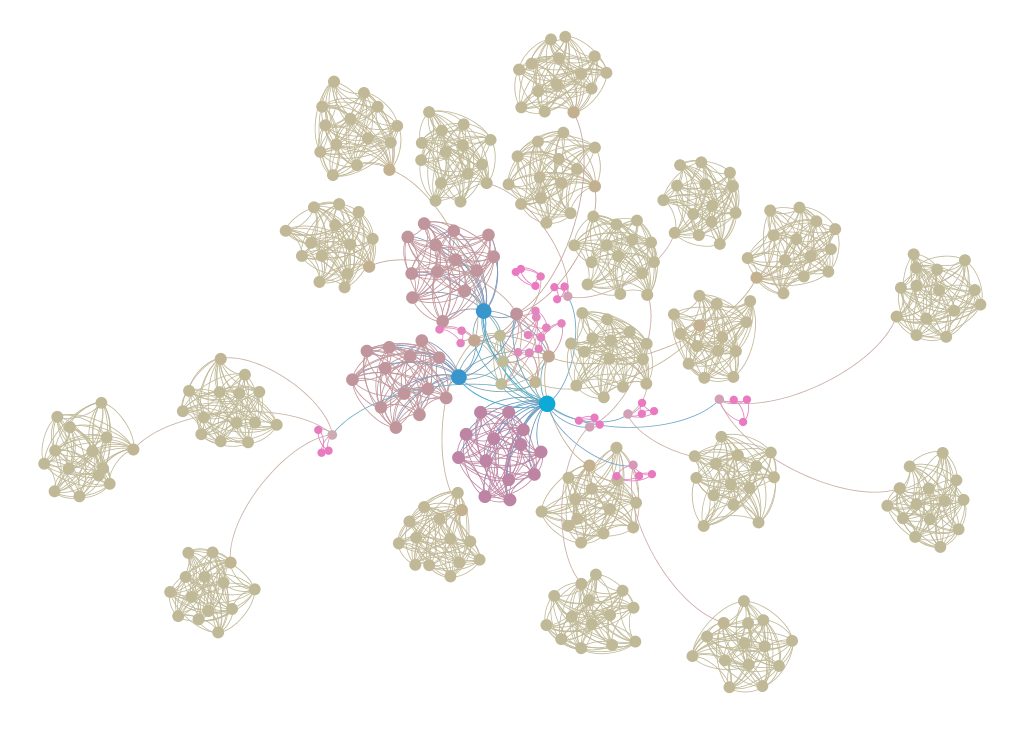
\includegraphics[width=15cm]{figure_2.png}
\caption{Information Network in ICM} \label{fig:Information Network in ICM}
\end{figure}

We calculate some properties of this network:

Then we turn to the main part of building up our model and using it for analysis. To deal with the complicated real problems, we first simplify them into two process. The first process is named as "output" and the second process is named "input". Like in the real world and in the problem, the "output" process refers to the situations where the staff leave his or her position. The "input" process, accordingly, refers to the combination of internal promotion and outsourcing recruitment. The formal models are presented in the next section. Based on this process division, we can easily see that the "input" process is where the Human Resource manager works his or her power to control and improve the company's current position.

\subsection{Terms and Notations}

In order to keep clear and consistent through the paper, we will settle down some fixed terms referring to some specific constituents. Besides, we will settle down some abbreviations for later use. The mathematical notation rules are also summed up in this section.

\paragraph{Terms and Abbreviations}
\begin{itemize}
\item Position: We use position to refer to all the nodes in the network.
\item Level of position: we use level of position to refer to the seven administrative levels (manager, supervisor or employee).
\item Abbreviations: we assign each level an abbreviation: SE-Senior Executive, JE -  Junior Executive, ES - Experienced Supervisor, IS - Inexperienced Supervisor, EE - Experienced Employee, IE - Inexperienced Employee, AC - Administrative Clerk
\end{itemize}

\paragraph{Mathematical Notation Rules}
\begin{itemize}
\item $t$: time is discrete and the minimum time interval is one month.
\item $\Omega^{(t)}$: the set of people who leave the company at the end of $t$. \item $\Theta^{(t)}$: the set of people who are recruited the company at the beginning of $t$. 
\item $\Gamma^{(t)}$: the set of people who work in the company at the beginning of $t$ after recruitment. It's obvious that the relation $\Gamma^{(t+1)}=\Gamma^{(t)}\bigcup \Theta ^{(t+1)} \backslash \Omega^{(t)}$ holds.
\item $f^{(t)}$: the mapping from $\Gamma^{(t)}$ to $V(G)$, which maps individual $i\in \Gamma^{(t)}$ to his position $f^{(t)}(i) \in V(G)$ at time $t$. $f^{(t)-1}$ is the inverse mapping.
\item $d(u,v)$: the distance between two nodes $u, v\in V(G)$, defined by the length of the shortest path connecting $u$ and $v$ in the graph.
\item $d_{ij}^{(t)}$: the distance between two individuals $i, j\in  \Gamma^{(t)}$ at $t$, defined by $d(f^{(t)}(i),f^{(t)}(j))$.
\end{itemize}


\section{Models}

(\textcolor{red}{need refinement}) We hold the intention to create a dynamic model which can be controlled by manipulating some of the parameters. Specially, we assume that the "output" process is largely determined by individual characteristics rather than company's policy. However, we also want to create a set of tools that human resource managers can use to deal with the possible staff problems. With these in mind, we design two models that capture the process of "output" with different emphasis and simulate three possible strategy for the human resource manager: purely recruiting, purely promoting and the "greedy" strategy. These models and simulations will help to solve the task 1-5 and even dig deeper insights about staff management. 

Next we begin to build the model from two aspects: "output", which means the resign of current staff, and "input", which means the recruitment of new staff.

We have several bold assumptions that are used in all our subsequent analysis:
\begin{itemize}
\item We assume that all the data given in the first table in the problem, whether it is mean or average, has no uncertainty. That is the mean or median salary or recruiting cost is a certain number.
\item \textcolor{red}{We assume that the information will only transmit through the information web we have set up.}
\end{itemize}

\subsection{Churn Model}

\subsubsection{Basic Set-ups}

In recent studies, Bayesian learning has been used to analyze information aggregation in social networks, in which individuals modify their decision based on previous outcomes of other individuals in the network. (\textcolor{red}{A cite is needed for the topic Bayesian Learning in Social Networks})

The typical Bayesian learning process can be described as follows: For any individual in the system, we suppose he has a world of two states. He is making decisions over these two states, with a probability. And this probability comes out of a distribution. The common set-up for this is the probability comes out of a Beta distribution,described by two parameters $\alpha$ and $\beta$. The later decision making process is based on a Bernoulli Distribution with a parameter $p$. This $p$ comes from the Beta distribution. If a person is put into an environment where all the people are considered the same to himself. He then uses Bayesian inference to "learn" about his true state and thus make decisions accordingly. The learning process is realized by changing the parameters in the Beta distribution.

In the light of this, We introduce a novel method to model the churn rate conceptually similarly to Bayesian learning. Specifically, we view leaving the position as a decision making process: suppose an individual $i$ decides whether \textit{to leave} or \textit{to stay} in a particular month $t$ based on a random variable $u_{i,t} \in \{0, 1\}$, where $u_{i,t} = 0$ indicates \textit{to leave}, otherwise \textit{to stay} is indicated. $u_{i, m}$ is drawn as follows:

\begin{enumerate}
\item Assume two hyperparameters $\alpha_{i, t}$ and $\beta_{i, t}$;
\item Draw 
  \begin{equation}
   p_{i, m} \sim \mathrm{Beta}(\alpha_{i, t}, \beta_{i, t})
   \label{eq:beta}
  \end{equation}
  where $\displaystyle \mathrm{Beta}(x; \alpha, \beta) = \frac{x^{\alpha - 1}(1-x)^{\beta - 1}}{\mathrm{B}(\alpha, \beta)}$, and $\mathrm{B}(\alpha, \beta)$ is the normalization constant.
\item Draw 
  \begin{equation}
	u_{i, t} \sim \mathrm{Bernoulli}(p_{i, t})
    \label{eq:bernoulli}
  \end{equation}
  where $\mathrm{Bernoulli}(x; p) = p^x(1-p)^{1-x}$ is the Bernoulli distribution.
\end{enumerate}

The distribution of $u_{i, t}$ is a specification of the Beta-Binomial distribution, which has mean $\displaystyle \frac{\alpha}{\alpha + \beta}$ and variance $\displaystyle\frac{\alpha\beta}{(\alpha+\beta)^2}$. 

Updating the hyperparameters $\alpha$ and $\beta$ can be viewed as a Bayesian learning process: an increase in $\alpha_i$ decreases $i$'s tendency to churn, while an increase in $\beta_i$ increases this tendency. Moreover, increasing $\alpha_i$ and $\beta_i$ reduces the variance of the Beta distribution, indicating that the individual has a better estimation of $p_i$. We also take the network structure into account, where the outcome of nearer individuals have more influence.

\subsubsection{Decision Making Process}

This distribution has good properties: on the one hand, the overall churn rate can be easily estimated using the hyperparameters of each individual; on the other hand, since the Beta distribution is the conjugate prior of the Bernoulli distribution, $\alpha$ and $\beta$ can be conveniently updated given observed results. For simplicity, please refer to Pattern Recognition and Machine Learning for more details.


\paragraph{Information Effect}
In this model, we capture the way an individual is influenced by other people's leaving using information flow. In other words, the event of one person leaves acts as a influential message, transmitting across the network built earlier. We call it information effect. We assume that the information effect will accumulate, that is, the churn news this month and last month will have an equal and add-up influence in shaping the listen's decision. In order to make the model easier to control, we add an assumption that the a piece of information's effect will expire after six months. This modeling technique can be justified by the psychological evidence (\textbf{where to find any???}) that . 

To formalize this process in mathematical expressions, we first define some metric to measure the information effect. 



Formally, the information effect on individual $i\in \Gamma{(t)}$ can be calculated as follows:

$$\displaystyle \sum_{\tau=t-6}^{t-1}\sum_{j\in \Omega^{(\tau)}}\frac{e_j^{(\tau)}}{d_{ij}^{(\tau)2}}$$

The ways that the model capturing the current situations of the company:
\begin{itemize}
\item The information for used for learning will transmit through the information network. It models the effect of connection.
\item The matching of people and positions can be modeled by introducing classification of people and positions, which will be discussed in detail later.
\item The "middle manager" having higher intrinsic churn rate can be modeled by inputting different $\alpha/ \beta$.
\item The required experience is model into the vacancy-filling model by setting a line for getting promoted
\item The steadily increasing churn rate can be modeled in two ways: An external impact represented by a slowly-decreasing $\alpha$, or An internal process represented by a slowly-increasing influence on $\beta$
\end{itemize}


The update process is described in Algorithm \ref{algo:bayes}:

\RestyleAlgo{boxed}
\begin{algorithm}[H]
 \KwData{The network $G$, and the churned individuals in the first month $\Omega^{(t)}$}

 initialize t = 0, $\alpha_{i,0}$ and $\beta_{i,0}$ for $\forall i \in \Gamma(t)$\;
 \While{True}{
   \For{$\forall i \in \Gamma(t) \backslash \Omega^{(t)}$}{
   	 $\hat{\alpha} = \hat{\beta} = 0$\;
     \For {$\forall j \in \Gamma(t) \backslash \Omega^{(t)}$} {
     	$\hat{\alpha} = \hat{\alpha} + 1 / d_{ij}^{(\tau)2}$\;
     }
     \For{$\forall j \in \Omega^{(t)}$} {
        $\hat{\beta} = \hat{\beta} + 1 / d_{ij}^{(\tau)2}$\;
     }
     
     $\alpha_i = \alpha_i + \frac{\hat{\alpha}}{\hat{\alpha} + \hat{\beta}}$\;
     $\beta_i = \beta_i + \frac{\hat{\beta}}{\hat{\alpha} + \hat{\beta}}$\;
   }
   $\Omega^{(t)} = \Phi$\;
   \For{$\forall i \in \Gamma(t)$} {
     Sample $u_{i,t}$ according to \ref{eq:beta} and \ref{eq:bernoulli}\;
     \eIf {$u_{i, t} = 0$} {
       $i$ choose to churn\;
       $\Omega^{(t+1)} = \Omega^{(t+1)} \and \{i\}$;
     }{
     	$i$ choose not to churn\;
     }
   }
   $t = t + 1$\;
 }
 \caption{Algorithm for the Bayesian Churn Model}
 \label{algo:bayes}
\end{algorithm}

\subsection{Vacancy-filling Model}

In this part, we consider the process of 


\subsubsection{A "baseline" Strategy}

To fulfill the first five tasks of modeling the current operation of the company, we model a "baseline" vacancy-filling . As described in the problem, the "naive" manager now has the following features:
\begin{itemize}
\item He does not read the annual evaluation report, thus does not know anything about the matching between staff and positions. In this way, he will not consider changing staff within one level.
\item His first choice is to choose to promote someone that has reached the experience requirement to fill the vacancy. If no person has reached the requirement, then he will post recruitment need for this position. In other words, he only post recruitment need after seeing there is a vacant position and no person can fill the vacancy.
\item If more than one person have meet the experience requirement, he randomly picks one from all these candidates.
\item If during the time the recruitment need is posted, he finds that there is one person's experience has reached the requirement. He will directly promote and cancel the recruitment post.
\item He will not promote a clerk because recruiting an inexperienced employee is cheaper and less time-consuming than recruiting a clerk. In other words, a "naive" manager never promotes a clerk.
\item His maximum effort for recruitment is around 8\%-10\% of the total number, as mentioned in the problem. When the number of vacant positions is higher than his maximum, he ranks the vacant positions from higher level to lower level. That is to say, he will first consider recruiting a manager rather than an employee when they are all vacant. The motivation behind this lies in that the time needed for recruiting a manager is much longer.
\end{itemize}



\subsubsection{Strategies}

\paragraph{Pure Strategies}
The most easily thought of strategies are the pure ones:
\begin{itemize}
\item Pure Promoting: Under this strategy, the HR manager exert no external recruiting and promote only qualified individuals 
\end{itemize}

\paragraph{Greedy Strategy}

The scheme for this "greedy" strategy can be described by the following rules:
\begin{itemize}
\item When there is a vacancy in the position, the HR manager will first rearrange the staff within the same tier to get a better \textbf{\Large{matching}}.
\item After this rearrangement, this strategy requires the HR manager to first seek opportunity to make promotions. The main reason is that promotion will save both the time and money needed for recruitment. However, any person getting promotion must first meet the experience requirement.
\item The above rule will not be obeyed for the situation where an inexperienced employee position is vacant. For recruiting a clerk costs more than recruiting an inexperienced employee directly.
\item \textit{The total number of recruitment is less than 37 (10\% of the total number 370 as mentioned in the tasks).}(\textbf{argued})
\item The recruitment will start only after observing a position is vacant and no person can be promoted to fill the vacancy. That is to say, the HR manager is "discreet". He doesn't believe in any prediction of the possible job vacancy under this strategy. In the meanwhile, he will place job vacancy in the higher level in higher order when considering recruiting. In other words, because of the upper limit of the total recruitment, there might be situations where vacant positions needing recruiting cannot be satisfied all. Then he will place the preceding order. The main consideration behind this lies in the recruitment time for higher tier is usually higher.
\end{itemize}

As we can see, supplement strategy effectively control the matching problem. Consider the company has been operating under this strategy for an enough long period of time, the friction will be all eliminated by this strategy because of the first step.

\paragraph{Prediction Strategy}


\paragraph{Matching Strategy}


\paragraph{Centrality Strategy}


\subsubsection{Model Modification Possibilities}

\paragraph{The Difference between Good News and Bad News}

\paragraph{Information Intensity}

Both in reality and in the context of this problem, a certain amount of experience is required for getting promotion. Usually, the higher tier to be promoted into, the longer the experience is needed. In the model, we assume that the required experience for promotion only takes into account the time length of being in the former level. E.g. only the time length of being in the level of junior manager set to be requirement for consideration of promoting senior manager. Suppose the experience requirement for each level of position is represented by $R_i, i = 1, 2...,7$. This can be a rich set of tools that the HR manager can use to control the organizational structure and even churn rate.

\paragraph{Modeling Matching and Frictions}



\section{Simulations}

\textbf{Added Assumptions for Simulation}

\subsection{Simulations with "Baseline" Strategy}


\subsection{Simulations with Other Strategies}

\subsection{Test the Effectiveness of Adjusting Experience Requirement}


\section{Model Applications}

\subsection{Measure Productivity}

To define a metric to measure this company's organizational productivity, we start from the individual level. This metric should incorporate the following three aspects:

\paragraph{Position Level}
Different levels of position surely make different contribution to the overall performance of a company. We reasonably assume the relative average annual salary of $i$'s position level, $S_i^{(t)}$ can properly reflect his actual level contribution.

\paragraph{Training experience}
Experience in his current position definitely contribute to one's productivity. We use the training cost the company spent on the individual since he began working in the current position as a proxy of his experience, denoted by $T_i^{(t)}*t_i^{(t)}$, where $T_i^{(t)}$ is the average annual training cost of the individual $i$'s position at time $t$.

\paragraph{Dissatisfaction}
Dissatisfaction is another important factor in determining an individual's productivity. An individual more unsatisfied with current situation tends to work less inefficiently, leading to lower productivity. We calculate $i$'s dissatisfaction $\sigma_i^{(t)}$ as:

$$\displaystyle \sigma_i^{(t)}=\sum_{\tau=t-t_i^{(t)}+1}^{t-1}e^{-(\tau-(t-1))}\sum_{j\in \Omega^{(\tau)}}\frac{1}{d_{ij}^{(\tau)2}}$$

We normalize $\sigma_i^{(t)}$ to the form of $\displaystyle \frac{1}{1+\alpha\ln{(1+\sigma_i^{(t)})}}$, so that $\lim\limits_{\sigma_i^{(t)}\rightarrow 0} \displaystyle \frac{1}{1+\alpha\ln{(1+\sigma_i^{(t)})}}=1$ and $\lim\limits_{\sigma_i^{(t)}\rightarrow \infty} \displaystyle \frac{1}{1+\alpha\ln{(1+\sigma_i^{(t)})}}=0$. Here, $\alpha$ is a control parameter, we set it to be $\displaystyle \frac{1}{3}$ in the following calculation in this part. We will carry on sensitivity analysis regarding to this parameter in later section.\\

Incorporating those three components, we can define the productivity of an individual $i$ at time $t$ as:
$$\displaystyle p_i^{(t)}=\frac{1}{1+\alpha\ln{(1+\sigma_i^{(t)})}}(S_i^{(t)}+T_i^{(t)}*t_i^{(t)})$$

To calculate organizational productivity, we use the weighted sum of individual's productivity: 
$$P^{(t)}=\sum\limits_{i\in\Gamma^{(t)}} w_i^{(t)}*p_i^{(t)}$$.

The weight $w_i^{(t)}$ is associated with information network structure. An individual in an important position in the network has more weight in calculating organizational productivity. Here we use the closeness centrality to reflect this importance, which is defined by:

$$\displaystyle w_i^{(t)}=\sum\limits_{v\in V(G)\backslash f^{(t)-1}(i)}\frac{d(v,f^{(t)-1}(i))}{370-1}$$

With this measure in hand, we can track the dynamic process of productivity change. Especially, we can calculate the direct effect and indirect effect associated with the resign of a specific individual.

We define the direct effect pf the resign on organizational productivity as the loss of the productivity due to the exit of these individuals. Total effect is the difference in organizational productivity immediately before and after the resign. The indirect effect is the difference between total effect and direct effect. We need to calculate the indirect effect very carefully to eliminate the effect on organizational productivity resulting from more training, the increase in satisfaction after promotion and the enter of new staff. Another way to think of the indirect effect is the loss of productivity caused by the increase of dissatisfaction of the remaining staff in this company. Explicitly, we have:

$$D^{(t)}_{effect}=\sum\limits_{i\in\Omega^{(t)}}w_i^{(t)}*p_i^{(t)}$$ $$I^{(t)}_{effect}=\sum\limits_{i\in\Gamma^{(t)}\backslash\Omega^{(t)}} w_i^{(t)}*(\frac{1}{1+\alpha\ln{(1+e^{-1}\sigma_i^{(t)})}}-\frac{1}{1+\alpha\ln{(1+\sigma_i^{(t+1)})}})(S_i^{(t)}+T_i^{(t)}*t_i^{(t)})$$

Using these definitions, we can calculate the loss of organizational productivity associated with the resign of staff and decompose it into direct effect and indirect effect. \textcolor{red}{For reason discussed before}, we report the results from the beginning of the second year.


\subsection{Budget Calculation}

In this part, we set up to consider the budget related to human capital the company is faced with. There are three components of the budget. Namely, they are the staff salaries, recruiting costs and staff training fees. To make calculation easier, as we assumed before, all individuals in the same level of position have the same annual salary and training cost, and the recruitment cost and time are also uniform in each level of position, which are given in Table 1 in the problem. All costs are induced uniformly distributed across the corresponding time span.

We explicitly run simulation of our company and the results are shown below:

\section{Team Science and Multi-layers}
There are several possible extensions to the models we have described before. These extensions are used to modify some of the bold but kind of restrictive assumptions made before and help to come closer to reality. Note that some of these new extensions need information about the real data of the company. Besides, being more precise means in the other direction that the extended models will not be as powerful and encompassing as the baseline models. Though the insights they are shedding lights on are basically the same.

\subsection{Incorporating Team Science}

\subsection{Incorporating Multi-layers}
In this section, we will take into consideration the progress made by rencent studies about multi-layer networks. 



\section{Sensitivity Analysis}


\section{Strengths and Weaknesses}

\section{Summary}

\bibliography{Reference}

\end{document}
